% !TEX root = BA-Bauer.tex
\subsection{Menü}
Die Menüführung ist ein essentieller Bestandteil für die intuitive Bedienbarkeit des Gerätes. Sie muss leicht für den Benutzer zu durchschauen sein und mit den begrenzten Möglichkeiten der C-Porgrammiersprache auch programmierbar sein. Für die Menüführung wird ein einfaches Modell aus mehreren Ebenen verwendet. Nach dem das Gerät gestartet und alle Schnittstellen initialisiert sind wird das Hauptmenü auf dem LCD-Display angezeigt. Der Inhalt des Display ist in Abbildung \ref{fig:lcdmain} zu sehen. Das Hauptmenü stellt Ebene 0, also die unterste Ebene des Menus dar. Zu beginn ist der erste Menüeintrag gewählt und wird mit einem Pfeil in der ersten Spalte des LCD-Displays markiert. Durch drehen des Encoders kann der Pfeil und damit der ausgewählte Eintrag verändert werden. Eine Drehung im Uhrzeigersinn verschiebt die Auswahl nach unten, eine Drehung gegen den Uhrzeigersinn nach oben. Ist die auszuführende Funktion mithilfe des Pfeils ausgewählt, so kann mit der Betätigung des Bestätigungs-Tasters die nächste Ebene des Menüs erreicht werden. Mithilfe des Zurück-Tasters kann zu der vorherigen Ebene zurückgekehrt werden. Je nach Auswahl werden die Inhalte aus Abbildung \ref{fig:lcdplay}, \ref{fig:lcdrec} oder \ref{fig:lcdset} angezeigt. Da auf dem LCD-Display lediglich vier Zeilen zu Anzeige zur Verfügung stehen sind Abbildung \ref{fig:lcdrec} und \ref{fig:lcdset} um die nicht sichtbaren Zeilen gestreckt. 
\begin{figure}[h]
	\begin{minipage}{.22\linewidth}
		\centering
		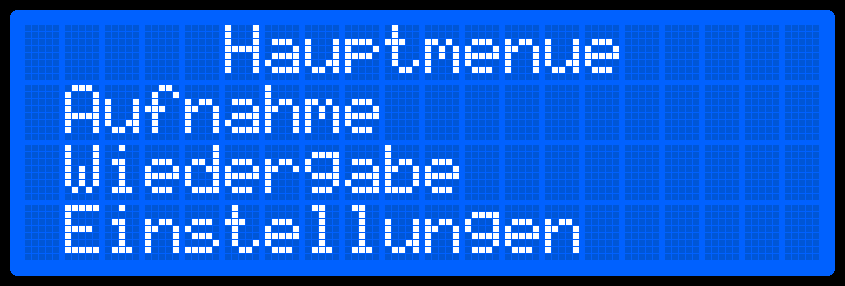
\includegraphics[width = \linewidth]{LCD-Screenshots/Hauptmenue}
		\caption{LCD-Hauptmenü}
		\label{fig:lcdmain}
	\end{minipage}
	\hfill
	\begin{minipage}{.22\linewidth}
		\centering
		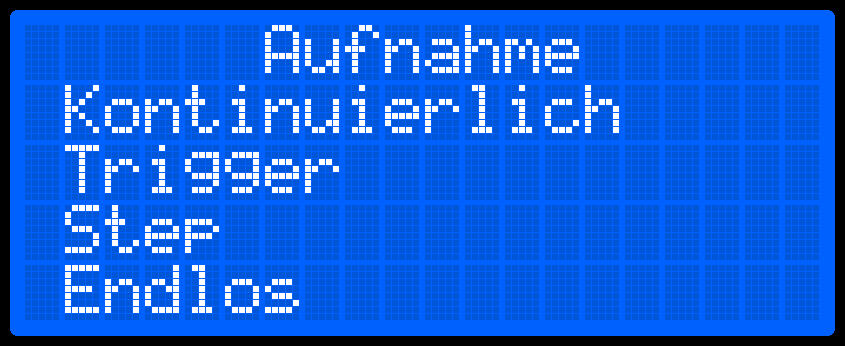
\includegraphics[width = \linewidth]{LCD-Screenshots/Aufnahme}
		\caption{LCD-Aufnahme}
		\label{fig:lcdrec}
	\end{minipage}
	\hfill
	\begin{minipage}{.22\linewidth}
		\centering
		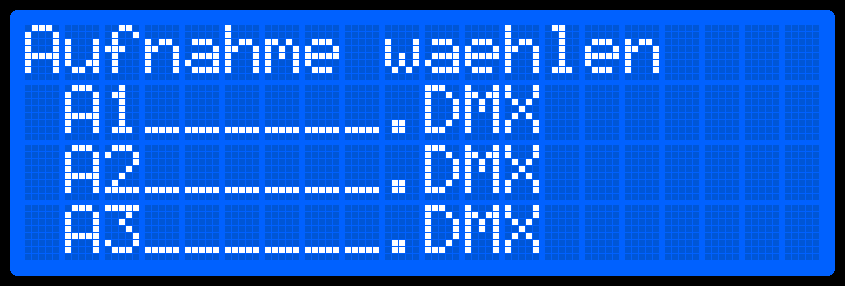
\includegraphics[width = \linewidth]{LCD-Screenshots/Wiedergabe}
		\caption{LCD-Wiedergabe}
		\label{fig:lcdplay}
	\end{minipage}
	\hfill
	\begin{minipage}{.22\linewidth}
		\centering
		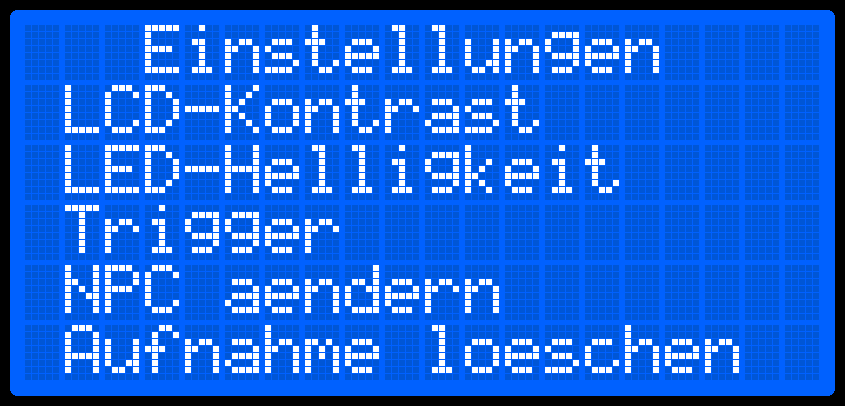
\includegraphics[width = \linewidth]{LCD-Screenshots/Einstellungen}
		\caption{LCD-Einstellungen}
		\label{fig:lcdset}
	\end{minipage}
\end{figure}
In Ebene 3 des Menüs befinden sich die tatsächlichen Funktionen zur Aufnahme und Wiedergabe der DMX-Daten und den Einstellungen. Im Hauptprogramm wird lediglich die Funktion $main\_menu(...)$ aufgerufen, um das Hauptmenü anzuzeigen. Die Zeichenketten, welche über das LCD-Display ausgegeben werden, sind in einem mehrdimensionalen $char$-Array definiert (Codeausschnitt \ref{code:menuarray}). Die erste Dimension des Arrays entspricht der Anzahl der anzuzeigenden Menuelemente, die zweite die Anzahl der zu beschreibenden Spalten des LCD-Displays. Es werden bewusst nur 19 Spalten der verfügbaren 20 mit den Menuelementen beschrieben, da vor jedem Element Platz freigehalten wird für den den Pfeil, der die aktuelle Auswahl anzeigt. Um willkürliche Zeichen, die sich eventuell noch in den Speicherzellen befinden, werden die nicht benötigten Zeichen mit Leerzeichen überschrieben.
\lstinputlisting[firstline = 13, firstnumber = 13, lastline = 18, language = C, caption = Definition Zeichenkettenarray für LCD-Display-Ausgaben, label = code:menuarray]{/Users/Felix/Documents/CubeMX/BPA-Code/Core/Src/menu.c}
Durch die Verwendung der Zeichenkettenarrays können die Menüeinträge einfach verändert oder erweitert werden. Abbildung \ref{fig:flusshauptmenu} zeigt den Ablauf der Funktion $main\_menu(...)$. Zunächst werden alle Inhalte vom Display entfernt und die Menüüberschrift ausgegeben. Die globale Variable der Position des Encoders wird auf den Initialwert 0 zurückgesetzt. Daraufhin werden die ersten drei Menüeinträge aus dem Zeichenkettenarray unterhalb der Menüüberschrift ausgegeben (Abbildung \ref{fig:lcdmain}). Der Wert der Encoderposition entspricht der aktuellen Auswahl des Benutzers. Inital gilt der erste Eintrag als ausgewählt. Um nicht bei jedem Durchlauf der Funktion den gesamten Displayinhalt erneut ausgeben zu müssen erfolgt eine Abfrage ob sich die Encoderposition geändert hat. Nur wenn er sich verändert hat, wird der Auswahlpfeil an der entsprechend resultierenden Stelle angezeigt. Ist der Enter-Taster betätigt, wird das nächste entsprechende Menü aufgerufen.
\begin{figure}[h]
	\centering
	\includegraphics[width = .4\linewidth]{menue}
	\caption{Flussdiagramm Hauptmenü}
	\label{fig:flusshauptmenu}
\end{figure}
Welche Menüfunktion aufgerufen wird, wird mithilfe $switch-case$-Anweisung der Encoderposition entschieden. Im Gegensatz zum Hauptmenü müssen die Funktionen aller anderen Menü-Ebenen mit einem $return$-Befehl oder durch erreichen des Endes der Funktion beendet werden, da andernfalls die Menüfunktionen rekursiv aufgerufen werden. Zwangsläufig entstehen daraus Speicherprobleme, da reservierter Speicherplatz durch den Aufruf der Funktionen nicht wieder freigegeben wird. Ist der Speicher voll, so kommt es bei einem nächsten Funktionsaufruf zum Überlauf des Speichers und dadurch zu Fehlfunktionen oder vollständigen Abbruch des Programms.